% Slides for 2025-05-13
% To create a slide, use the following:
% \begin{frame}{TITLE}
%     BODY
% \end{frame}

% To create a slide with a bullet list, use the following:
% \begin{frame}{TITLE}
%     \begin{itemize}
%         \item ITEM 1
%         \item ITEM 2
%     \end{itemize}    
% \end{frame}

% To create a slide with numbered list, use the following:
% \begin{frame}{TITLE}
%     \begin{enumerate}
%         \item ITEM 1
%         \item ITEM 2
%     \end{enumerate}
% \end{frame}

% To create a slide with a graphic:
% 1. Add the graphic to this folder (named picture.png)
% 2. Use the following:
% \begin{frame}{TITLE}
%     \centering
%     \includegraphics[height=0.7\textheight,width=0.7\textwidth,keepaspectratio]{picture.png}
% \end{frame}

% To create a slide with two columns, use the following:
% \begin{frame}{TITLE}
%     \begin{columns}
%         \begin{column}{0.5\textwidth}
%             COLUMN 1 BODY
%         \end{column}
%         \begin{column}{0.5\textwidth}
%             COLUMN 2 BODY
%         \end{column}
%     \end{columns}
% \end{frame}

\begin{frame}{Rust Pipeline}
  \begin{columns}[c]
      \column{0.30\textwidth}
        \centering
        
\includegraphics[height=0.45\textheight,keepaspectratio]{./images/img1.png}
  
      \column{0.44\textwidth}
        \centering
        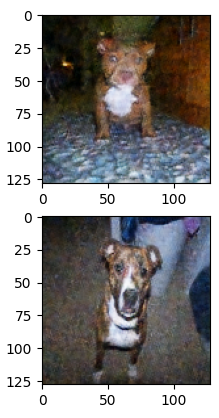
\includegraphics[height=0.45\textheight,keepaspectratio]{./images/img3.png}
      \column{0.30\textwidth}
        \centering
        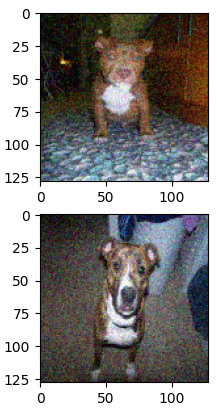
\includegraphics[height=0.45\textheight,keepaspectratio]{./images/img2.png}
  \end{columns}
      \begin{enumerate}
        \item Segment around 100 test images with truths
        \item Compare normalized pixel difference from truths (with old python pipeline)
        \item Look into hipify-perl converting Mitsuba + Dr.Jit CUDA code to HIP
    \end{enumerate}
\end{frame}

\begin{frame}{Tom - Underwater Renderer}
    \begin{enumerate}
      \item Attempted implement simple FP64 gelu with CubeCL in rust
      \item Discovered that FP64 achieved by converting to FP32, doing calculation, then sale back to FP64; loses accuracy
      \item CubeCL HIP seems to be the only HIP binding for rust; AMD GPU only, requires rocWMMA or WMMA Intrinsics (FP16 only); also unsafe since raw bindings
      \item Switching to C++ as Rust has limited support and benifit because of the unsafe GPU calls
      \item Reading PBRT book, looking into drjit-core and HIPIFY. Possible simple renderer from the ground up?
      \item rocWMMA requires MI1/2/300 series for FP64 runs, unable to test running code on GPU yet
    \end{enumerate}
\end{frame}
